\documentclass{article}

\usepackage{arxiv}

\usepackage[utf8]{inputenc} % allow utf-8 input
\usepackage[T1]{fontenc}    % use 8-bit T1 fonts
\usepackage{hyperref}       % hyperlinks
\usepackage{url}            % simple URL typesetting
\usepackage{booktabs}       % professional-quality tables
\usepackage{amsfonts}       % blackboard math symbols
\usepackage{nicefrac}       % compact symbols for 1/2, etc.
\usepackage{microtype}      % microtypography
\usepackage{lipsum}
\usepackage[dvipsnames]{xcolor}
\usepackage{graphicx}
\usepackage{float}
\usepackage{subcaption}

\title{Particle Pollution Estimation using Images}

\author{
  Yash Jalan \thanks{M.S. Scientific Computing} \\
  Courant Institute of Mathemetics\\
  New York University\\
  New York, NY 10012 \\
  \texttt{yj627@nyu.edu} \\
}

\begin{document}
\maketitle

\begin{abstract}
Outdoor images can often reveal important atmospheric information. It is not hard to determine by looking at an outdoor image whether the atmosphere in the image is hazy (smoky, foggy) or clear. It can be useful for the general public to be able to determine how hazy or how polluted the atmosphere actually is. In this paper, a new technique to estimate the PM-2.5 concentration levels in the air using images is studied. The technique combines computer vision techniques of dehazing and convolutional neural networks to approximate the pollution concentration level in the air using an image. The image dehazing algorithm via a dark channel is used to obtain a transmission function which estimates the pixel-wise haze density in the image. The extracted transmission function serves as the main feature in the final convolutional neural network to approximate PM-2.5 levels in the image. This is achieved by pretraining a U-Net with input as hazy colored outdoor images and the haze density images as output. The mean square error of this prior network is close to $10^{-5}$. The weights of the pretrained U-Net are transferred to the final network consisting of a LeNet-5 sitting on top of a U-Net to approximate the PM-2.5 concentration level in the image. On the 20 percent validation dataset of 866 images, this method achieves approximately an average mean square error of 260 in 400 epochs, which is not all that bad as PM-2.5 concentrations in the images range between 0 and 1000. Additionally, a lot of the images collected using Instagram do not have accurate date and times associated with them, and hence do not have the correct corresponding PM-2.5 concentration readings.
\end{abstract}

\keywords{Haze\and PM-2.5 \and CNN \and Dark  Channel Prior \and U-Net \and LeNet-5 \and MSE \and More}

\section{Introduction}

Dependence on fuel, as a source of energy via combustion, has increased over the years. The process of combustion (burning fuel, wood, etc.) produces fine particles called PM-2.5, which are less than 2.5 micrometers in diameter. Increased concentration and density of airborne PM-2.5 can cause and trigger respiratory diseases. In many urban areas in developing nations especially, where there exists many motor vehicles, industries and people, PM-2.5 concentration is high. Typically, PM-2.5 is accurately determined and measured by expensive devices inaccessible to the general public. High PM-2.5 concentration in the air leads to low visibility (haze). Often we hear people looking around and being able to determine the presence of pollution. Human eye however cannot accurately distinguish between haze caused by fog and PM-2.5 concentrations  and also cannot accurately estimate the level of  PM-2.5 concentration just by observing the atmosphere around. In order to increase awareness about the air pollution levels and the harm that it causes, it is good idea to develop an easily accessible and cheap mechanism that the general public can use to be better able to determine the PM-2.5 concentration around them. This paper presents a technique using images to determine the PM-2.5 concentration levels in real time. With increasing accessibility to mobile devices and their increased computational capabilities and ability to capture high quality photos, people can use this technique to capture image(s) of their surroundings and have a better idea about the PM-2.5 concentration level around them.

\section{Related Work}
\label{sec:related work}

There has been some previous work which have used images to estimate or classify PM-2.5 concentration levels. Wang et al. \cite{realtime} and Liu et al. \cite{PP} use domain specific knowledge to model scattering of light and accordingly generate features as input to a regression model to determine haze level or air quality or PM concentration levels. Li’s et al. \cite{Usergen} proposed method also relies on modeling light propagation to produce an estimate but uses combination of a depth map obtained using a deep convolutional neural field and a transmission function obtained using a dark channel prior to find correlation between the derived features and the PM-2.5 concentration levels. Wang et al. \cite{realtime} and Liu et al. \cite{PP} additionally require a depth map of the image. While Wang et al. \cite{realtime} also requires a sequence of the same image as input, the model proposed in Liu et al. \cite{PP} is trained specifically for three single scene images. Bo et al. \cite{PPconv}, Zhang et al. \cite{EAPconv} and Chakma et al. \cite{IBAQconv} use different deep convolutional neural networks to estimate or classify the PM-2.5 concentration levels. While Bo et al. \cite{PPconv} combines the output of the CNN on the images with weather information in a regression model to produce the final estimate, Zhang et al. \cite{EAPconv} and Chakma et al. \cite{EAPconv} simply feed a CNN to the input images to produce a result. All three deep neural network approaches do not provide any understanding or intuition as to why the network learns the correct features and moreover, are not very accurate.
This paper tries to find the middle path between domain specific models in \cite{realtime},\cite{PP},\cite{Usergen} and more general deep neural network models in \cite{PPconv},\cite{EAPconv},\cite{IBAQconv} to estimate the PM-2.5 concentration level in an image. This paper uses a dark channel prior to generate a transmission function to estimate the pixel-wise haze density in the image \cite{dcp}, which is used as the main feature in the final deep CNN to produce more accurate real-time pollution estimations using images.

\section{Datasets}
\label{sec:Datasets} 
The final dataset consists of two parts: single scene outdoor images of Beijing and Shanghai and multiple scene outdoor images of Delhi. In total, there are 4332 images and their corresponding PM-2.5 concentration levels in the dataset.
\subsection{Single Scene}
This dataset consists of images from Beijing and Shanghai. The Beijing images are of the exact same outdoor scene captured at different times of the day and days of the year. There are in total 327 images of Beijing. Similarly, 1885 images of the Oriental Pearl Tower in Shanghai City captured at different times of the day and days of the year exist \cite{PP}. The date and times of the captured images are exact and the PM-2.5 concentrations obtained from US Mission China \footnote{\url{http://www.stateair.net/web/historical/1/1.html}} are matched with the date and time of the image.

\begin{figure}[H]
\centering
\begin{subfigure}{.5\textwidth}
  \centering
  \includegraphics[width=.7\linewidth]{2014_04_24_0700_mod.jpg}
  \caption{Single-scene image of Beijing}
\end{subfigure}%
\begin{subfigure}{.5\textwidth}
  \centering
  \includegraphics[width=.85\linewidth]{201412291415_mod.jpg}
  \caption{Single-scene image of Shanghai}
\end{subfigure}
\caption{Single-scene image dataset}
\label{Single-scene image dataset}
\end{figure}

\subsection{Multiple Scenes}
The second part of the dataset consists of 2120 outdoor images of Delhi. The images (includes per second frames of videos) along with their upload date, time and exact location if available are scraped from Instagram. Upload times of the images are checked to see if they make sense, i.e. if the image is of daytime then the upload time should be of daytime and similarly for nighttime. If the upload time indicates night (day) and the image is clearly of daytime (nighttime), then the upload time is subtracted by 12 hours. The timing are important as they are required to match with the times of the PM-2.5 concentration levels, which are obtained from the  Govt. of India sensors \footnote{\url{https://app.cpcbccr.com/ccr/#/caaqm-dashboard-all/caaqm-landing/caaqm-comparison-data}}. The dates don't matter so much as research from Shiva, Prof. Subramanian (yet to be published?) show that the daily pollution levels in Delhi follow a pattern. So, the previous day's PM-2.5 concentration level will look similar to the next day's PM-2.5 concentration level and will only vary based on the time of the day or over a period of months. Since there exists PM-2.5 concentration data from multiple pollution sensors across Delhi, an average of the "hotspots" are taken for images with no specific location given and for images with specific location given, data from the closest or closest two monitoring station(s) are taken.

\begin{figure}[H]
\centering
\begin{subfigure}{.5\textwidth}
  \centering
  \includegraphics[width=.7\linewidth]{29404124_1815319278773605_7075081274305544192_n.jpg}
  \caption{example image of Delhi}
\end{subfigure}%
\begin{subfigure}{.5\textwidth}
  \centering
  \includegraphics[width=.7\linewidth]{23164879_288983588172607_9209412044523044864_n.jpg}
  \caption{example image of Delhi}
\end{subfigure}

\begin{subfigure}{.5\textwidth}
  \centering
  \includegraphics[width=.7\linewidth]{14709613_1686312078351865_8768219556335321088_n.jpg}
  \caption{JLN stadium}
\end{subfigure}%
\begin{subfigure}{.5\textwidth}
  \centering
  \includegraphics[width=.7\linewidth]{14540616_322525878139543_3555842517150728192_n.jpg}
  \caption{example image of Delhi}
\end{subfigure}
\caption{Multiple-scene image dataset}
\label{Multiple-scene image dataset}
\end{figure}

\newpage
\section{Methodology}
\label{sec:Methodology}

\subsection{Preprocessing}

Directly feeding a CNN with hazy outdoor colored input images will likely make the network learn the contours of the objects in the scene and will likely produce unintuitive results such as in (\cite{PPconv},\cite{EAPconv},\cite{IBAQconv}). For a CNN to be able to learn the correct features, specifically the colors of the background and foreground, preprocessing the images by generating intuitive features is essential before feeding it as input to a network. Here are some preprocessing steps that were taken as part of this paper:
\begin{itemize}
    \item The difference between the denoised (via OpenCV) and original image to detect fine particles in the image.
    \item A pixel-wise depth estimate of the image to reflect the density of haze of foreground objects. This was generated using unsupervised Monocular Depth Estimation with Left-Right Consistency \cite{monodepth} and implemented using existing codebase on GitHub \footnote{\url{https://github.com/mrharicot/monodepth}}.
    \item A pixel-wise haze density approximation obtained from a transmission function using computer vision algorithm of dehazing an image via a dark channel prior \cite{dcp}. The self-implemented algorithm is slow because it doesn't make use of a GPU. 
    \item Standardizing the images by subtracting from each image each channel's mean and dividing by the standard deviation (mean and std are computed with respect to the entire image dataset) to induce an underlying normal distribution.
\end{itemize}
To determine causal relationship between the preprocessed images, generated features and the PM-2.5 concentration levels, strong correlation is a good indicator whether the "intuitive" features will give good results or not. A combination of all the above features were tried and correlations between the quantiles of the features and PM-2.5 levels were computed for each dataset separately. The strongest correlations are obtained for the haze density feature, summarized below.
\begin{center}
\begin{tabular}{ c c c c c c}
 Dataset & Quantile & rank correlation & correlation & rank p-value & p-value\\ 
 Beijing & 100 & -0.68237 & -0.70803 & 1.352e-35 & 1.986e-50\\  
 Shanghai & 90 & -0.48599  & -0.52572 & 1.492e-113 & 6.197e-136 \\
 Beijing \& Shanghai & 80 & -0.4059  & -0.3045 & 3.465e-89 & 4.563e-49\\
 Delhi & 100 & -0.01402  & -0.23487 & 0.518 & 5.843e-28 \\
\end{tabular}
\end{center}
It is clear from the table above that there exists a negatively sloped linear relationship between the generated haze density of an image and the image's PM-2.5 concentration level. For the single scene accurately timed images from China, the correlations confirm that haze density feature is infact "intuitive". The inaccurate readings of the PM-2.5 concentration levels because of inaccurate timings, and filtering of images, the haze density feature of Instagram images of Delhi do not show monotonic relationship with the PM-2.5 concentration level, but the Pearson correlation does show there exists slight non-montonic relationship. The p-value with respect to the Peason correlation for the Delhi dataset is extrememly small, indicating that the haze density feature is infact statistically significant. Note that correlation only confirms a linear relationship between the input and output, however, since the model being studied uses nonlinear combinations of the input feature, the final results are not reflected by this measure. A linear combination of the depth estimating feature and haze density feature produced slightly better correlations for the Beijing dataset, and similar or slightly worse results for the other datasets (similar demonstration in \cite{Usergen}). Since the haze density image produced using a transmission function is a rough estimate of the depth \cite{dcp} and the results of the two competing features vary only slightly, the final model uses only the pixel-wise haze density feature.

\subsubsection{Dark Channel Prior}
He et al. \cite{dcp} statistically observe that for a haze-free image it is very likely that at least one of the color channels has very low intensity pixel values. Because of scattering of light, all color channels of hazy images have high intensity pixel values (indicated by a bright white-ish color). Using this observation, light scattering model, and intuition that the pixel-values of the dark channel (color channel with lowest intensity on non-sky patches) of the hazy image is a rough estimate haze density, He et al. propose a single-image dehazing algorithm which requires computing the transmission function, an estimate of the density of pixel values as part of the final algorithm. The underlying light propagation model in the algorithm requires computing the atmospheric light to compute the transmission function, giving more importance to objects closer in the z-direction to the camera. The density of haze will be larger for objects closer to the camera, which follows from the intuition that reflection of light against closest objects are the best indicators of the haze. So, indirectly the transmission function also computes a rough estimate of the depth of objects in the image.
\begin{figure}[H]
\centering
\begin{subfigure}{.5\textwidth}
  \centering
  \includegraphics[width=.5\linewidth]{2014_04_24_0700_mod.jpg}
  \caption{original image}
\end{subfigure}%
\begin{subfigure}{.5\textwidth}
  \centering
  \includegraphics[width=.5\linewidth]{2014_04_24_0700_mod_trans.jpg}
  \caption{estimate of haze density}
\end{subfigure}

\begin{subfigure}{.5\textwidth}
  \centering
  \includegraphics[width=.7\linewidth]{201412291415_mod.jpg}
  \caption{original image}
\end{subfigure}%
\begin{subfigure}{.5\textwidth}
  \centering
  \includegraphics[width=.7\linewidth]{201412291415_mod_trans.jpg}
  \caption{estimate of haze density}
\end{subfigure}

\begin{subfigure}{.5\textwidth}
  \centering
  \includegraphics[width=.4\linewidth]{29404124_1815319278773605_7075081274305544192_n.jpg}
  \caption{original image}
\end{subfigure}%
\begin{subfigure}{.5\textwidth}
  \centering
  \includegraphics[width=.4\linewidth]{29404124_1815319278773605_7075081274305544192_n_trans.jpg}
  \caption{estimate of haze density}
\end{subfigure}

\begin{subfigure}{.5\textwidth}
  \centering
  \includegraphics[width=.4\linewidth]{23164879_288983588172607_9209412044523044864_n.jpg}
  \caption{original image}
\end{subfigure}%
\begin{subfigure}{.5\textwidth}
  \centering
  \includegraphics[width=.4\linewidth]{23164879_288983588172607_9209412044523044864_n_trans.jpg}
  \caption{estimate of haze density}
\end{subfigure}
\caption{Per-image transmission function obtained via Dark Channel prior to generate pixel-wise haze densities}
\label{Per-image transmission function obtained via Dark Channel prior to generate pixel-wise haze densities}
\end{figure}

\newpage
\subsection{Pretraining}
The pixel-wise haze densities of the entire image dataset is computed using the dark channel prior algorithm. It is possible to use this feature directly as input to a network, but that has two main drawbacks. One, the final application will require to first generate the haze denisity of the input hazy image which is a computationally expensive process possibly requiring use of a GPU. Two, it will remove the possibility of the machine learning rich hidden details in the original hazy image, hence making the model more restrictive. A nice work-around solution to this is to use a pretraining CNN for the machine to learn to generate haze densities of an image on the fly. A U-Net (popularly used for segmentation on medical images) is used for this task. The architecture of the U-Net can be observed in [Figure \ref{U-Net}]. The input image size differs slightly. The images are resized to 256 by 256 and the output is of same size except it consists of only one channel. The input images are standardized using mean and standard deviation computed with respect to the entire dataset. This helps (empirically tested) the network converge faster. With the entire dataset as input for training, after only 5 epochs, the mean square error is less than $10^{-5}$.

\subsection{Model}

The final model used to approximate the PM-2.5 concentration levels in an image consists of U-Net [Figure \ref{U-Net}] joined at the end to a LeNet-5 [Figure \ref{LeNet-5}]. It takes standardized outdoor hazy colored images as input and produces an approximation of PM-2.5 concentration levels in the images. The input to the first LeNet-5 layer is the output from the U-Net which is a single channeled image (haze density estimate) of size 256 by 256. Using transfer learning, the weights of the pretrained U-Net are transferred to this final network so that the CNN can leverage the pretrained U-Net to generate the haze-density feature of the input image. The final output of this combination of U-Net and LeNet-5 CNN is a single number, which is the PM-2.5 concentration level of the image.

\begin{figure}[H]
  \centering
  \includegraphics[width=0.7\linewidth]{u-net-architecture.png}
  \caption{U-Net}
  \label{U-Net}
\end{figure}
\begin{figure}[H]
  \centering
  \includegraphics[width=0.65\linewidth]{The-LeNet-5-Architecture.png}
  \caption{LeNet-5}
  \label{LeNet-5}
\end{figure}

\section{Results}
Both the pretraining and final model are trained with loss function as mean square error. The final dataset (consisting of both single scene and multiple scene images) is divided randomly (using a constant random seed generator) into 80 percent training and 20 percent validation set. With optimizer as Adam (algorithm is based on AdaGrad, which uses adaptive gradients for each iteration and is known to work well for large datsets) and learning rate as $0.0001$, the mean square error for training set reduces to single digit after 145 epochs. After 145 epochs, the mean square error on training and validation set stabilizes to approximately 5 and 270 respectively. The lowest mean square error for the validation set reaches 252.840. The PM-2.5 concentration levels range between 0 and 1000. The mean and standard deviation of the PM-2.5 levels of the entire dataset is 105.99 and 110.91 respectively, which means that PM-2.5 varies a lot from image to image.
\begin{table}[H]
\centering
\begin{tabular}{|l|l|l|}
\hline
 Metric & Training set & Validation set\\ \hline
 MSE & 2.560 & 252.840 \\ \hline
 MAE & 4.874 & 18.735  \\ \hline
\end{tabular}
\end{table}
The other related papers either use different image datasets (mainly multiple-scene Beijing dataset) for evaluation or treat the task as a classification task, so the results are very hard to compare. The table above and the figures below summarize the resulting errors of this paper's model.

\begin{figure}[H]
\centering
\begin{subfigure}{.5\textwidth}
  \centering
  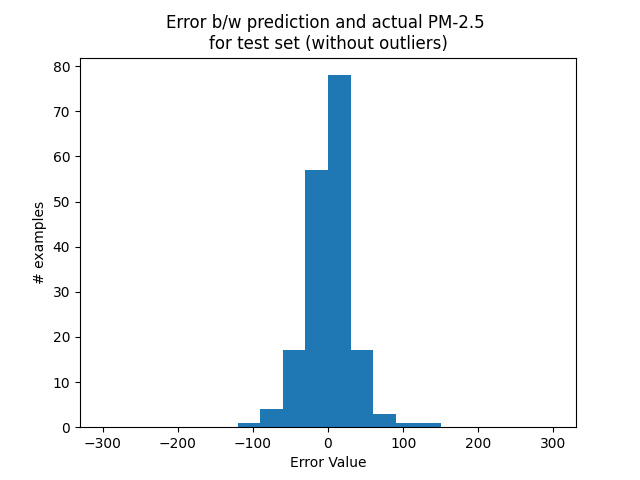
\includegraphics[width=.8\linewidth]{err_full.png}
  \caption{Entire dataset}
\end{subfigure}%
\begin{subfigure}{.5\textwidth}
  \centering
  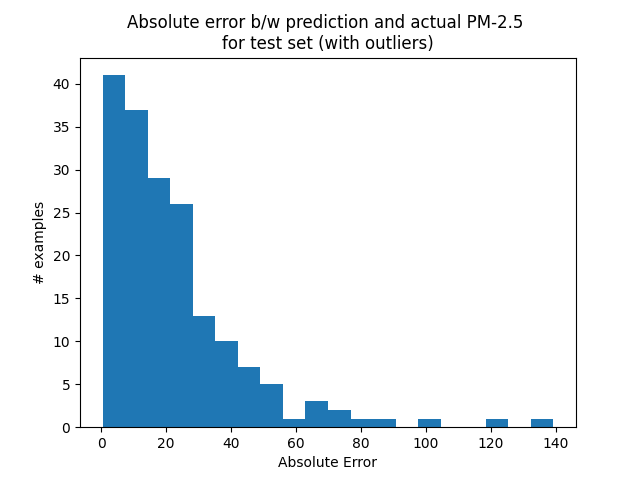
\includegraphics[width=.8\linewidth]{err_val.png}
  \caption{Validation set}
\end{subfigure}

\begin{subfigure}{.5\textwidth}
  \centering
  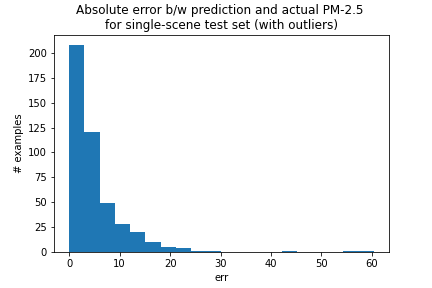
\includegraphics[width=.8\linewidth]{err_china.png}
  \caption{Single-scene China images}
\end{subfigure}%
\begin{subfigure}{.5\textwidth}
  \centering
  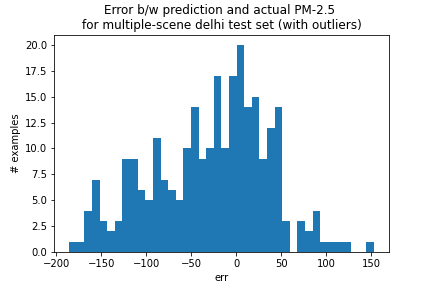
\includegraphics[width=.8\linewidth]{err_delhi.png}
  \caption{Multiple-scenes Delhi images}
\end{subfigure}
\caption{Histograms of the difference between the predicted and actual PM-2.5}
\label{Histograms of the difference between the predicted and actual PM-2.5}
\end{figure}
The shapes of the histograms of the errors (difference between the actual and predicted PM-2.5) above indicate an underlying normal distribution of the errors. The mean and standard deviation of the errors are summarized in the table below. 
\begin{table}[H]
\centering
\begin{tabular}{|l|l|l|l|l|l|}
\hline
 Error & Entire dataset & Validation & Single-scene (China) & Multiple-scene (Delhi)\\ \hline
 mean & -1.021 & -5.634 & -1.629 & -0.382 \\ \hline
 std & 28.786 & 62.377 & 8.360 & 40.318 \\ \hline
\end{tabular}
\end{table}
The relatively low standard deviation of the errors show that the model is able to, with good accuracy and certainty approximate the PM-2.5 concentration levels for the single-scene image dataset. The relatively low mean, high standard deviation and the presence of extremely incorrect results in the validation image dataset and the multiple-scene Instagram image dataset of Delhi indicate that even though the model is able to approximate relatively well for many images in the sets, there exist some outliers which skew the errors. Below are some examples of images and their actual and predicted PM-2.5 concentration levels that better illustrate the model's strengths and shortcomings.

\begin{figure}[H]
\centering
\begin{subfigure}{.5\textwidth}
  \centering
  \includegraphics[width=.6\linewidth]{bad/37672324_279736822801516_8078809865750839296_n.jpg}
  \caption{actual=43.07, pred=238.91}
\end{subfigure}%
\begin{subfigure}{.5\textwidth}
  \centering
  \includegraphics[width=.5\linewidth]{bad/47253026_157163518610448_2136220676494070664_n.jpg}
  \caption{actual=389.7, pred=190.1}
\end{subfigure}

\begin{subfigure}{.5\textwidth}
  \centering
  \includegraphics[width=.55\linewidth]{bad/23422033_150729815537066_7609480750454276096_n.jpg}
  \caption{actual=421.03, pred=73.44}
\end{subfigure}%
\begin{subfigure}{.5\textwidth}
  \centering
  \includegraphics[width=.5\linewidth]{bad/43984815_1888703911227305_1679019398446941429_n.jpg}
  \caption{actual=378.1, pred=101.18}
\end{subfigure}

\begin{subfigure}{.5\textwidth}
  \centering
  \includegraphics[width=.35\linewidth]{bad/46848680_526463111201161_7042018332420154853_n.jpg}
  \caption{pred=209.37, actual=732.85}
\end{subfigure}%
\begin{subfigure}{.5\textwidth}
  \centering
  \includegraphics[width=.6\linewidth]{bad/29908859_405140603286124_1262735481834045440_nframe6.jpg}
  \caption{pred=121.71, actual=121.67}
\end{subfigure}

\begin{subfigure}{.5\textwidth}
  \centering
  \includegraphics[width=.4\linewidth]{good/2014_06_10_0618_mod.jpg}
  \caption{pred=79.6, actual=76.0}
\end{subfigure}%
\begin{subfigure}{.5\textwidth}
  \centering
  \includegraphics[width=.6\linewidth]{good/201412301445_mod.jpg}
  \caption{pred=84.97, actual=85.0}
\end{subfigure}
\caption{Examples to illustrate where model failed, succeeded}
\label{Examples to illustrate where model failed, succeeded}
\end{figure}
When using nonlinear approximations and deep neural networks, it is hard to reason why the model does well for certain examples and why it doesn't for the others. For instance, in Fig \ref{Examples to illustrate where model failed, succeeded} (c), it is discernible even to human eye that the pollution level is extreme, but the model under approximates, whereas in the same figure (f), humans will never be able to tell what the pollution level in the photo, but the model predicts this with high accuracy. There also exists issues in the problem statement and/or the PM-2.5 readings of the image dataset, as image (e) doesn't "seem" polluted, but the actual PM-2.5 value says otherwise. For non-sky images with consistently accurate PM-2.5 readings such as the single-scene image dataset, the model performs fairly well.

\section{Improvements \& Future Work}

There are several drawbacks and shortcoming to this study, which can be further improved. This paper is unable to properly reason the results of the model. The error, especially for Instagram images of Delhi, shows random behaviour with large standard deviation. Thus, the Instagram image dataset itself could be a severe bottleneck. Following are some ways the model in this paper can be improved and better understood:

\begin{itemize}
    \item Using unprocessed (eg. non-filtered) images with accurate date and times. This would map the image to the correct PM-2.5 estimates and would possibly lead to lower, more consistent and understandable error.
    \item Using images with plenty of foreground objects with very little background sky. Images with a lot of sky lead to a relatively poor density map as the dark channel prior density algorithm assumes non-sky images.
    \item Including weather features in the model could improve prediction as the model could then distinguish between haze caused by foggy weather and haze caused by particulate matter.
    \item Using mean absolute error as loss function would probably reduce the significance of outliers in the model.
    \item Very little hyperparameter tuning was done. Dropout layers, batch normalization, longer training, grid searching for the hyperparameters of the CNN could increase accuracy.
\end{itemize}

Here is the link to the repository of this project: \url{https://github.com/yashjal/particle-detection}.

\bibliographystyle{unsrt}  
%\bibliography{references}  %%% Remove comment to use the external .bib file (using bibtex).
%%% and comment out the ``thebibliography'' section.

%%% Comment out this section when you \bibliography{references} is enabled.
\begin{thebibliography}{1}

\bibitem{realtime}
Haoqian Wang, Xin Yuan, Xingzheng Wang, Yongbing Zhang, Qionghai Dai.
\newblock Real-time Air Quality Estimation Based on Color
Image Processing.
\newblock In {\em IEEE Conference on Visual Communications and Image Processing}, pp. 326–329. IEEE, 2014.

\bibitem{PP}
Chenbin Liu, Francis Tsow, Yi Zou, Nongjian Tao.
\newblock Particle Pollution Estimation Based on Image
Analysis.
\newblock In {\em PloS one 2016}. 2016.

\bibitem{Usergen}
Yucheng Li, Jifei Huang, and Jiebo Luo. 
\newblock Using user generated online photos to estimate and monitor air pollution in major cities.
\newblock In {\em Proceedings of the 7th ACM international conference on Internet Multimedia Computing and Service}, pp. 79. ACM, 2015.

\bibitem{PPconv}
Qirong Bo, Wenwen Yang, Nabin Rijal, Yilin Xie, Jun Feng, Jing Zhang.
\newblock Particle Pollution Estimation from Images using Convolutional Neural Network and Weather Features.
\newblock In {\em 2018 IEEE International Conference on Image Processing}. IEEE, 2018.

\bibitem{EAPconv}
Chao Zhang, Junchi Yan, Changsheng Li, Xiaoguang Rui, Liang Liu, and Rongfang Bie.
\newblock On Estimating Air Pollution from Photos Using
Convolutional Neural Network.
\newblock In {\em Proceedings of the 24th ACM international conference on Multimedia}, pages 297-301. ACM, 2016.

\bibitem{IBAQconv}
Avijoy Chakma, Ben Vizena, Tingting Cao, Jerry Lin, and Jing Zhang.
\newblock Image Based Air Quality Analysis Using Deep
Convolutional Neural Network.
\newblock In {\em 2017 IEEE International Conference on Image Processing}. IEEE, 2017.

\bibitem{dcp}
Kiaming He, Jian Sun, and Xiaoou Tang. 
\newblock Single image haze removal using dark channel prior. CVPR, 2009.

\bibitem{monodepth}
Clément Godard, Oisin Mac Aodha, and Gabriel J. Brostow.
\newblock Unsupervised Monocular Depth Estimation with Left-Right Consistency. CVPR, 2017.


\end{thebibliography}


\end{document}
